\section{GIÁ TRỊ LƯỢNG GIÁC CỦA MỘT GÓC TỪ $0^\circ$ ĐẾN $180^\circ$}
\subsection{TÓM TẮT LÝ THUYẾT}
\subsubsection{Giá trị lượng giác của một góc}
\begin{itemize}
	\item [\iconMT] \indam{Định nghĩa:} Với mỗi góc $\alpha$ $(0^\circ\le \alpha \le 180^\circ )$, ta xác định duy nhất một điểm $M$ trên nửa đường tròn đơn vị sao cho $\widehat{xOM}=\alpha $. Giả sử điểm $M$ có tọa độ $M(x_0;y_0 )$, khi đó ta có định nghĩa
	\begin{gachsoc}
		\immini{
			\begin{itemize}
				\item \textbf{sin} của góc $\alpha$ là $y_0$, kí hiệu $\sin\alpha = y_0$.
				\item \textbf{cô-sin} của góc $\alpha$ là $x_0$, kí hiệu là $\cos\alpha = x_0$.
				\item \textbf{tang} của góc $\alpha$ là $\dfrac{y_0}{x_0} \left(x_0\neq 0\right)$, kí hiệu là $\tan\alpha = \dfrac{y_0}{x_0}$.
				\item \textbf{cô-tang} của góc $\alpha$ là $\dfrac{x_0}{y_0} \left(y_0\neq 0\right)$, kí hiệu là $\cot\alpha = \dfrac{x_0}{y_0}$.
			\end{itemize}
			Các số $\sin\alpha$, $\cos\alpha$, $\tan\alpha$, $\cot\alpha$ được gọi chung là các \textit{giá trị lượng giác} của góc $\alpha$.
		}{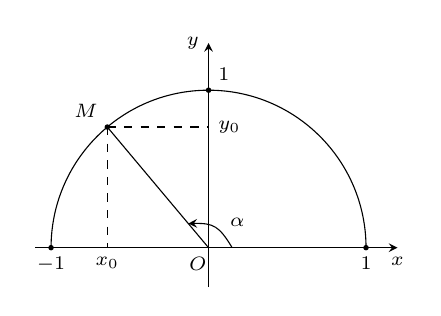
\begin{tikzpicture}[>=stealth,font=\scriptsize]
				\draw[->] (-2.2,0) -- (2.4,0) node[below]{$x$};
				\draw[->] (0,-.5) -- (0,2.6) node[left]{$y$};
				\fill[black] (.1,0) node[below left]{$O$}
				(-2,0) circle(1pt) node[below]{$-1$}
				(2,0) circle(1pt) node[below]{$1$}
				(0,2) circle(1pt) node[above right]{$1$};
				\draw (2,0) arc (0:180:2cm);
				\path (130:2cm) coordinate (M);
				\fill (M) circle(1pt);
				\draw[dashed] (M) node[above left]{$M$} -- (M|- 0,0) node[below]{$x_0$};
				\draw[dashed] (M) -- (M -|0,0) node[right]{$y_0$};
				\draw (0,0) -- (M);
				\draw[->] (0.3,0) to [bend right,looseness=1.3] (130:0.4cm);
				\fill (0.15,0.15) node[above right]{$\alpha$};
		\end{tikzpicture}}
	\end{gachsoc}
	\item [\iconMT] \indam{Bảng giá trị lượng giác của góc đặc biệt}
	\begin{center}
		\renewcommand{\arraystretch}{2}
		\begin{tabular}{|c|c|c|c|c|c|c|}
			\hline
			& $0^\circ$ & $30^\circ$ & $45^\circ$ & $60^\circ$ & $90^\circ$ & $180^\circ$\\
			\hline
			$\sin \alpha$  & $0$ & $\dfrac{1}{2}$ & $\dfrac{\sqrt{2}}{2}$ & $\dfrac{\sqrt{3}}{2}$ & $1$ & $0$\\
			\hline
			$\cos \alpha$  & $1$ & $\dfrac{\sqrt{3}}{2}$ & $\dfrac{\sqrt{2}}{2}$ & $\dfrac{1}{2}$ & $0$ & $-1$\\
			\hline
			$\tan \alpha$ & $0$ & $\dfrac{1}{\sqrt{3}}$ & $1$ & $\sqrt{3}$ & $\big|\big|$ & $0$\\
			\hline
			$\cot \alpha$ & $\big|\big|$ & $\sqrt{3}$ & $1$ & $\dfrac{1}{\sqrt{3}}$ & $0$ & $\big|\big|$\\
			\hline
		\end{tabular}
	\end{center}
	\item \indam{Các công thức cơ bản} 
	\begin{tcolorbox}[colframe=orange,colback=white,boxrule=0.2mm]
		\begin{multicols}{3}
			\begin{enumerate}[1)]
				\item $\sin^2\alpha + \cos^2\alpha = 1$; 
				\item $\tan \alpha=
				\dfrac{\sin\alpha}{\cos\alpha}$; 
				\item $\cot \alpha=
				\dfrac{\cos\alpha}{\sin\alpha}$;
				\item $\tan \alpha\cdot \cot \alpha = 1$;
				\item $1+\tan^2\alpha=\dfrac{1}{\cos^2\alpha}$;
				\item $1+\cot^2\alpha=\dfrac{1}{\sin^2\alpha}$.
			\end{enumerate}
		\end{multicols}
	\end{tcolorbox}
\end{itemize}
\subsubsection{Mối quan hệ giữa các giá trị lượng giác}
\begin{itemize}
	\item [\iconMT] \indam{Hai góc bù nhau:} Trên hình bên ta có dây cung $NM$ song song với trục $Ox$ và nếu $\widehat{xOM}=\alpha $ thì $\widehat{xON}=180^\circ-\alpha $. Ta có $y_{M}=y_{N}=y_0,$ $x_{M}=-x_{N}=x_0$. Do đó
	\begin{gachsoc}	
		\immini{
			\begin{itemize}
				\item $\sin (180^\circ-\alpha )=\sin \alpha$
				\item $\cos (180^\circ-\alpha )=-\cos \alpha$
				\item $\tan (180^\circ-\alpha )=-\tan \alpha$
				\item $\cot (180^\circ-\alpha )=-\cot \alpha$
			\end{itemize}
		}{\begin{tikzpicture}[scale=1, font=\footnotesize,>=stealth,x=2cm,y=2cm]
				\def\x{0.715}
				\def\a{44}
				\pgfmathsetmacro{\y}{\x*tan(\a)}
				\draw[->] (-1.3,0)--(1.3,0) node [below]{$x$};
				\draw[->] (0,-0.2)--(0,1.3) node [left]{$y$};
				\node at (0,0) [below left]{$O$};
				\draw (1,0) arc (0:180:2cm);
				\fill (1,0) node[below]{$1$} circle(1pt);
				\fill (-1,0) node[below]{$-1$} circle(1pt);
				\fill (0,1) node[above left]{$1$} circle(1pt);
				\fill (\x,0) node[below]{$x_0$} circle(1pt);
				\fill (-\x,0) node[below]{$-x_0$} circle(1pt);
				\fill (\a:1) node[above right]{$M$} circle(1pt);
				\fill (180-\a:1) node[above left]{$N$} circle(1pt);
				\fill (0,\y) node[above right]{$y_0$} circle(1pt);
				\draw[dashed] (\x,0)|-(0,\y);
				\draw[dashed] (-\x,0)|-(0,\y);
				\draw (44:1)--(0,0)--(136:1);
				\draw (0.3,0) arc (0:\a:0.6cm);
				\node at (0,0)[shift={(25:0.2)}]{\tiny{$\alpha$}};
				\draw (0.2,0) coordinate (A) -- (0,0) coordinate (B) -- (136:0.6 cm) coordinate (C) pic [draw, double, angle radius = 9mm] {angle = A--B--C}; 
				\draw (0.25,0.55)node{\tiny{$180^\circ-\alpha$}};
		\end{tikzpicture}}
	\end{gachsoc}
	\item [\iconMT] \indam{Hai góc phụ nhau:} Hình vẽ bên, hai điểm $M$ và $N$ ứng với hai góc phụ nhau $\alpha$ và $90^\circ-\alpha$ ($\widehat{xOM}=\alpha$, $\widehat{xON}=90^\circ-\alpha$ )
	\begin{gachsoc}
		\immini{
			\begin{itemize}
				\item $\cos \left( 90^\circ-\alpha  \right) = \sin \alpha$
				\item $\sin \left(90^\circ-\alpha  \right) = \cos \alpha$
				\item $\tan \left(90^\circ-\alpha  \right) = \cot \alpha$
				\item $\cot \left( 90^\circ-\alpha  \right) = \tan \alpha$
			\end{itemize}
		}{
			\begin{tikzpicture}[scale=1, font=\footnotesize,>=stealth,x=2cm,y=2cm]
				\def\x{0.866}
				\def\a{30}
				\pgfmathsetmacro{\y}{\x*tan(\a)}
				\draw[->] (-1.3,0)--(1.3,0) node [below]{$x$};
				\draw[->] (0,-0.2)--(0,1.3) node [left]{$y$};
				\node at (0,0) [below left]{$O$};
				\draw (1,0) arc (0:180:2cm);
				\fill (1,0) node[below]{$1$} circle(1pt);
				\fill (-1,0) node[below]{$-1$} circle(1pt);
				\fill (0,1) node[above left]{$1$} circle(1pt);
				\fill (\x,0) node[below]{$x_0$} circle(1pt);
				\fill (\a:1) node[above right]{$M$} circle(1pt);
				\fill (90-\a:1) node[above right]{$N$} circle(1pt);
				\fill (0,\y) node[left]{$y_0$} circle(1pt);
				\draw[dashed] (\x,0)|-(0,\y);
				\draw[dashed] (\y,0)|-(0,\x);
				\draw (\a:1)--(0,0)--(90-\a:1);
				\draw (0.3,0) arc (0:\a:0.6cm);
				\node at (0,0)[shift={(15:0.25)}]{\tiny{$\alpha$}};
				\draw (0.2,0) coordinate (A) -- (0,0) coordinate (B) -- (90-\a:0.6 cm) coordinate (C) pic [draw, double, angle radius = 9mm] {angle = A--B--C}; 
				\draw (0.65,0.14)node{\tiny{$90^\circ-\alpha$}};
		\end{tikzpicture}}
	\end{gachsoc}
\end{itemize}

\subsection{RÈN LUYỆN KĨ NĂNG GIẢI TOÁN}
\begin{dang}{Tính giá trị lượng giác của một góc, một biểu thức}
	Để tính giá trị lượng giác của một góc hoặc một biểu thức
	\begin{itemize}
		\item \textbf{Đối với góc đặc biệt:} ta dùng bảng giá trị lượng giác của góc đặc biệt.
		\item \textbf{Đối với góc còn lại:} ta dùng hai góc bù nhau, hai góc phụ nhau với những góc lớn hơn $90^\circ$.
	\end{itemize}
	\begin{enumerate}[1)]
		\item Bảng giá trị lượng giác của góc đặc biệt
		\begin{center}
			\renewcommand{\arraystretch}{2}
			\begin{tabular}{|c|c|c|c|c|c|c|}
				\hline
				& $0^\circ$ & $30^\circ$ & $45^\circ$ & $60^\circ$ & $90^\circ$ & $180^\circ$\\
				\hline
				$\sin \alpha$  & $0$ & $\dfrac{1}{2}$ & $\dfrac{\sqrt{2}}{2}$ & $\dfrac{\sqrt{3}}{2}$ & $1$ & $0$\\
				\hline
				$\cos \alpha$  & $1$ & $\dfrac{\sqrt{3}}{2}$ & $\dfrac{\sqrt{2}}{2}$ & $\dfrac{1}{2}$ & $0$ & $-1$\\
				\hline
				$\tan \alpha$ & $0$ & $\dfrac{1}{\sqrt{3}}$ & $1$ & $\sqrt{3}$ & $\big|\big|$ & $0$\\
				\hline
				$\cot \alpha$ & $\big|\big|$ & $\sqrt{3}$ & $1$ & $\dfrac{1}{\sqrt{3}}$ & $0$ & $\big|\big|$\\
				\hline
			\end{tabular}
		\end{center}
		\textbf{Chú ý:} Trong bảng, kí hiệu $\big|\big|$ để chỉ giá trị lượng giác không xác định.
		\item Hai góc bù nhau
		\begin{itemize}
			\item $\sin (180^\circ-\alpha )=\sin \alpha$
			\item $\cos (180^\circ-\alpha )=-\cos \alpha$
			\item $\tan (180^\circ-\alpha )=-\tan \alpha$
			\item $\cot (180^\circ-\alpha )=-\cot \alpha$
		\end{itemize}
		\item Hai góc phụ nhau
		\begin{itemize}
			\item $\cos \left( 90^\circ-\alpha  \right) = \sin \alpha$
			\item $\sin \left(90^\circ-\alpha  \right) = \cos \alpha$
			\item $\tan \left(90^\circ-\alpha  \right) = \cot \alpha$
			\item $\cot \left( 90^\circ-\alpha  \right) = \tan \alpha$
		\end{itemize}
	\end{enumerate}
\end{dang}

\begin{vd}%[0H4N1-2]%[Dự án đề cương 3 khối NH24-25 - Đợt 2 - Quan Ón]%[SGK CTST]
	Tìm các giá trị lượng giác của góc $120^\circ$.
	\loigiai{
		\immini{
			Lấy điểm $M$ trên nửa đường tròn đơn vị sao cho $\widehat{xOM}=120^\circ$.\\
			Ta có $\widehat{MOy}=120^\circ-90^\circ=30^\circ$. \\
			Ta tính được tọa độ điểm $M$ là $\left(-\dfrac{1}{2} ; \dfrac{\sqrt{3}}{2}\right)$.\\
			Vậy theo định nghĩa, ta có
			$$ \sin 120^\circ=\dfrac{\sqrt{3}}{2};\quad \cos 120^\circ=-\dfrac{1}{2}; \quad \tan 120^\circ=-\sqrt{3};\quad \cot 120^\circ=-\dfrac{\sqrt{3}}{3}. $$
		}
		{\begin{tikzpicture}[scale=1.2, font=\footnotesize,line join=round, line cap=round, >=stealth,x=2cm,y=2cm]
				\def\x{0.71}
				\def\a{60}
				\pgfmathsetmacro{\y}{\x*tan(\a)}
				\draw[->] (-1.3,0)--(1.3,0) node [below]{$x$};
				\draw[->] (0,-0.2)--(0,1.3) node [left]{$y$};
				\node at (0,0) [below left]{$O$};
				\draw (1,0) arc (0:180:2cm);
				\fill (1,0) node[below]{$1$} circle(1pt);
				\fill (-1,0) node[below]{$-1$} circle(1pt);
				\fill (0,1) node[above left]{$1$} circle(1pt);
				%	\fill (\x,0) node[below]{$x_0$} circle(1pt);
				%	\fill (-\x,0) node[below]{$N$} circle(1pt);
				%	\fill (\a:1) node[above right]{$M$} circle(1pt);
				\fill (180-\a:1) node[above left]{$M$} circle(1pt);
				%	\fill (0,\y) node[right]{$P$} circle(1pt);
				%	\draw[dashed] (-\x,0)|-(0,\y);
				\draw (0,0)--(120:1);
				\draw (0.3,0) arc (0:180-\a:0.6cm);
				\node at (0,0)[shift={(50:0.53)}]{$120^\circ$};
		\end{tikzpicture}}
	}
\end{vd}

\begin{vd}%[0H4H1-2]%[Dự án đề cương 3 khối NH24-25 - Đợt 2 - Quan Ón]
	Tính giá trị đúng của các biểu thức sau (không dùng máy tính cầm tay).
	\begin{multicols}{2}
		\begin{enumerate}
			\item $A=\cos 0^\circ + \cos 40^\circ + \cos 120^\circ + \cos 140^\circ$;
			\item $B=\cos 15^\circ + \cos 35^\circ - \sin 75^\circ - \sin 55^\circ$.
		\end{enumerate}
	\end{multicols}
	\loigiai
	{
		\begin{enumerate}
			\item Ta có
			\allowdisplaybreaks
			\begin{eqnarray*}
				A &=& \cos 0^\circ + \cos 40^\circ + \cos 120^\circ + \cos 140^\circ\\
				&=& \cos 0^\circ + \cos 40^\circ + \cos\left(180^\circ - 60^\circ\right) + \cos\left(180^\circ - 40^\circ\right)\\
				&=& \cos 0^\circ + \cos 40^\circ - \cos 60^\circ - \cos 40^\circ\\
				&=& \left( \cos 40^\circ - \cos 40^\circ \right) + \cos 0^\circ - \cos 60^\circ\\
				&=& 0 +  1 - \dfrac{1}{2}\\
				&=& \dfrac{1}{2}.
			\end{eqnarray*}
			\item Ta có
			\allowdisplaybreaks
			\begin{eqnarray*}
				B &=& \cos 15^\circ + \cos 35^\circ - \sin 75^\circ - \sin 55^\circ \\
				&=& \cos 15^\circ + \cos 35^\circ - \sin\left(90^\circ-15^\circ\right) - \sin\left(90^\circ-35^\circ\right)\\
				&=& \cos 15^\circ + \cos 35^\circ - \cos 15^\circ - \cos 35^\circ \\
				&=& 0.
			\end{eqnarray*}
		\end{enumerate}
	}
\end{vd}

\begin{dang}{Rút gọn, chứng minh biểu thức}
	Dùng các kết quả cơ bản sau đây kết hợp với hai góc bù nhau và hai góc phụ nhau.
	\begin{multicols}{3}
		\begin{enumerate}[1)]
			\item $\sin^2\alpha + \cos^2\alpha = 1$; 
			\item $\tan \alpha=
			\dfrac{\sin\alpha}{\cos\alpha}$; 
			\item $\cot \alpha=
			\dfrac{\cos\alpha}{\sin\alpha}$;
			\item $\tan \alpha\cdot \cot \alpha = 1$;
			\item $1+\tan^2\alpha=\dfrac{1}{\cos^2\alpha}$;
			\item $1+\cot^2\alpha=\dfrac{1}{\sin^2\alpha}$.
		\end{enumerate}
	\end{multicols}
\end{dang}

\begin{vd}%[0H4H1-2]%[Dự án đề cương 3 khối NH24-25 - Đợt 2 - Quan Ón]%[TL PNL 2025]
	Không dùng bảng số hay máy tính cầm tay, tính giá trị của các biểu thức sau:
	\begin{multicols}{2}
		\begin{enumerate}
			\item $\sin^2 60^\circ+\cos^2 120^\circ+\cos^2 0^\circ-\tan ^260^\circ+\cot ^2135^\circ$;
			\item $\tan 25^\circ\cdot \tan 45^\circ\cdot \tan 115^\circ$.
		\end{enumerate}
	\end{multicols}
	\loigiai{
		\begin{enumerate}
			\item Ta có
			\allowdisplaybreaks
			\begin{eqnarray*}
				&& \sin^2 60^\circ+\cos^2120^\circ+\cos^2 0^\circ-\tan^2 60^\circ+\cot^2 135^\circ\\
				&=& \sin^2 60^\circ + \left(\cos 120^\circ\right)^2+\left(\cos 0^\circ\right)^2-\left(\tan 60^\circ\right)^2+\left(\cot 135^\circ\right)^2\\
				&=& \sin^2 60^\circ + \left[\cos \left(180^\circ-60^\circ\right)\right]^2+1-\left(\sqrt{3}\right)^2+\left[\cot \left(180^\circ-45^\circ\right)\right]^2\\
				&=& \sin^2 60^\circ +\left(\cos 60^\circ\right)^2 + 1-\left(\sqrt{3}\right)^2+\left(-\cot 45^\circ\right)^2 \\
				&=& \left[\sin^2 60^\circ + \cos^2 60^\circ\right] + 1-\left(\sqrt{3}\right)^2+\left(\cot 45^\circ\right)^2\\
				&=& 1 + 1-\left(\sqrt{3}\right)^2 + 1^2  \\
				&=& \dfrac{1}{4}.
			\end{eqnarray*}
			\item Ta có
			\allowdisplaybreaks
			\begin{eqnarray*}
				\tan 25^\circ\cdot \tan 45^\circ\cdot \tan 115^\circ &=& \tan 25^\circ\cdot \tan 45^\circ\cdot \tan\left(180^\circ - 65^\circ\right)\\
				&=& \tan 25^\circ\cdot \tan 45^\circ\cdot \left(-\tan 65^\circ\right)\\
				&=& -\tan 25^\circ\cdot \tan 45^\circ\cdot  \tan 65^\circ \\
				&=& -\tan 25^\circ\cdot \tan 45^\circ\cdot \tan\left(90^\circ - 25^\circ\right)\\
				&=& -\tan 25^\circ\cdot \tan 45^\circ\cdot \cot 25^\circ\\
				&=& -\left(\tan 25^\circ \cdot \cot 25^\circ\right)\tan 45^\circ \\
				&=& -1\cdot 1 \\
				&=& -1.
			\end{eqnarray*}
		\end{enumerate}
	}
\end{vd}

\begin{vd}%[0H4H1-3]%[Dự án đề cương 3 khối NH24-25 - Đợt 2 - Quan Ón]
	Cho $A$, $B$, $C$ là các góc của tam giác. Chứng minh các đẳng thức sau
	\begin{multicols}{2}
		\begin{enumerate}
			\item $\sin\left(A+B\right)=\sin C$;
			\item $\sin\dfrac{A+B}{2}=\cos\dfrac{C}{2}$.
		\end{enumerate}
	\end{multicols}
	\loigiai{
		Do $A$, $B$, $C$ là các góc của tam giác nên ta có $A+B+C=180^\circ$.
		\begin{enumerate}
			\item Ta có $A+B+C=180^\circ\Rightarrow A+B=180^\circ-C$.\\
			Từ đó suy ra $\sin\left(A+B\right)=\sin \left(180^\circ-C\right)=\sin C$.
			\item Ta có $A+B+C=180^\circ\Rightarrow \dfrac{A+B}{2}=\dfrac{180^\circ-C}{2}=90^\circ-\dfrac{C}{2}$.\\
			Từ đó suy ra $\sin\dfrac{A+B}{2}=\sin\left(90^\circ-\dfrac{C}{2}\right)= \cos\dfrac{C}{2}$.
		\end{enumerate}
	}
\end{vd}

\begin{dang}{Tính giá trị lượng giác với điều kiện góc cho trước}
	\begin{itemize}
		\item Nếu $\alpha$ là góc nhọn thì các giá trị lượng giác của $\alpha$ đều dương.
		\item Nếu $\alpha$ là góc tù thì $\sin\alpha>0$, $\cos\alpha<0$, $\tan\alpha<0$, $\cot\alpha<0$.
		\item $\tan\alpha$ chỉ xác định khi $\alpha \neq 90^\circ$.
		\item $\cot\alpha$ chỉ xác định khi $\alpha \neq 0^\circ$ và $\alpha\neq 180^\circ$.
	\end{itemize}
\end{dang}

\begin{vd}%[0H4H1-2]%[Dự án đề cương 3 khối NH24-25 - Đợt 2 - Quan Ón]
	Tính các giá trị lượng giác còn lại của góc $\alpha$, biết
	\begin{multicols}{2}
		\begin{enumerate}
			\item $\sin \alpha =\dfrac{1}{3}$ và $90^\circ<\alpha <180^\circ$;
			\item $\cos \alpha =\dfrac{3}{5}$ và $0^\circ <\alpha <90^\circ$;
			\item $\tan \alpha =\sqrt{3}$ và $0^\circ <\alpha <90^\circ$.
		\end{enumerate}
	\end{multicols}
	\loigiai{
		\begin{enumerate}
			\item Ta có $\cos^2 \alpha=1-\sin^2\alpha = 1-\dfrac{1}{9}=\dfrac{8}{9} \Rightarrow \cos \alpha = \pm \dfrac{2\sqrt{2}}{3}$.\\
			Do $90^\circ<\alpha <180^\circ$ nên $\cos \alpha <0$, suy ra $\cos \alpha = - \dfrac{2\sqrt{2}}{3}$
			\begin{itemize}
				\item  $\tan \alpha = \dfrac{\sin \alpha}{\cos \alpha}=-\dfrac{1}{2\sqrt{2}}$.
				\item  $\cot \alpha = \dfrac{1}{\tan \alpha}=-2\sqrt{2}$.
			\end{itemize} 
			\item Ta có $\sin^2 \alpha=1-\cos^2\alpha = 1-\dfrac{9}{25}=\dfrac{16}{25} \Rightarrow \sin \alpha = \pm \dfrac{4}{5}$.\\
			Do $0^\circ <\alpha <90^\circ$ nên $\sin \alpha >0$, suy ra $\sin \alpha = \dfrac{4}{5}$
			\begin{itemize}
				\item  $\tan \alpha = \dfrac{\sin \alpha}{\cos \alpha}=\dfrac{3}{4}$.
				\item  $\cot \alpha = \dfrac{1}{\tan \alpha}=\dfrac{4}{3}$.
			\end{itemize} 
			\item Ta có $\cos^2 \alpha=\dfrac{1}{1+\tan^2 \alpha}= \dfrac{1}{4} \Rightarrow \cos \alpha =\pm \dfrac{1}{2}$.\\
			Do $0^\circ <\alpha <90^\circ$ nên $\cos \alpha >0$, suy ra $\cos \alpha =  \dfrac{1}{2}$.
			\begin{itemize}
				\item $\tan\alpha = \dfrac{\sin\alpha}{\cos\alpha} \Rightarrow \sin\alpha = \tan\alpha\cdot\cos\alpha =  \dfrac{\sqrt{3}}{2}$.
				\item $\cot\alpha = \dfrac{1}{\tan \alpha}=\dfrac{1}{\sqrt{3}}$.
			\end{itemize} 
	\end{enumerate}}
\end{vd}

\subsection{Bài tập rèn luyện}
\ind{PHẦN I.} \inden{Câu trắc nghiệm nhiều phương án lựa chọn. Mỗi câu hỏi học sinh chỉ chọn một phương án.}\\
\setcounter{ex}{0}
\Opensolutionfile{ans}[ans/0H4-Bai1-TN]

\begin{ex}%[0H4H1-2]%[Lớp 10-HK1-THPT Chuyên Lê Quý Đôn - Ninh Thuận]%[Lê Hải Phụng]
	\immini{Biết rằng điểm $M(a;b)$ thoả mãn $\widehat{MOx}=30^\circ$ như hình vẽ.
		Khi đó giá trị của $a$ bằng
		\choice
		{$\dfrac{4}{5}$}
		{$\dfrac{\sqrt{2}}{2}$}
		{\True $\dfrac{\sqrt{3}}{2}$}
		{$\dfrac{1}{2}$}}{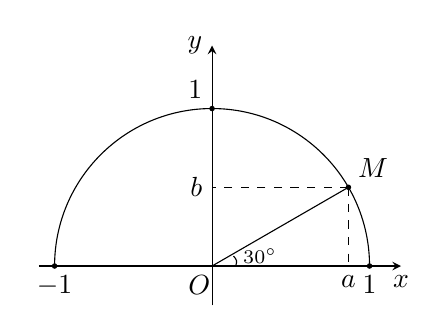
\begin{tikzpicture}[>=stealth]
			\draw[->] (-2.2,0) -- (2.4,0) node[below]{$x$};
			\draw[->] (0,-.5) -- (0,2.8) node[left]{$y$};
			\fill[black] (.1,0) node[below left]{$O$}
			(-2,0) circle(1pt) node[below]{$-1$}
			(2,0) circle(1pt) node[below]{$1$}
			(0,2) circle(1pt) node[above left]{$1$};
			\draw (2,0) arc (0:180:2cm);
			\path (30:2cm) coordinate (M);
			\fill[black] (M) circle(1pt);
			\draw[dashed] (M) node[above right]{$M$} -- (M|- 0,0) node[below]{$a$};
			\draw[dashed] (M) -- (M -|0,0) node[left]{$b$};
			\draw (0,0) -- (M);
			\draw[-] (0.3,0) to [bend right,looseness=1.3] (25:0.3cm) node[right]{\scriptsize $30^\circ$};
	\end{tikzpicture}}
	\loigiai{
		Ta có $a=\cos30^\circ=\dfrac{\sqrt{3}}{2}$.
	}
\end{ex}

\begin{ex}%[0H4N1-2]%[Dự án đề cương 3 khối NH24-25 - Đợt 2 - Quan Ón]
	\textit{(Trích đề thi GHKI - Trường THPT Tân Bình - Tp.HCM - Năm học 2024-2025)}\\
	Với mỗi góc $\alpha$ $\left(0^\circ\leq\alpha\leq180^\circ\right)$, xác định môt điểm $M\left(x_0;y_0\right)$ duy nhất nằm trên nửa đường tròn đơn vị sao cho $\widehat{xOM}=\alpha$. Khẳng định nào sau đây là \textbf{sai}?	
	\choice
	{$\sin\alpha=y_0$}
	{$\cos\alpha=x_0$}
	{$\tan\alpha=\dfrac{y_0}{x_0}$ $\left(x_0\neq 0\right)$}
	{\True$\cot\alpha=\dfrac{x_0}{y_0}$}
	\loigiai{
		Khẳng định sai $\cot\alpha=\dfrac{x_0}{y_0}$ do thiếu điều kiện $y_0\neq0$.
	}
\end{ex}

\begin{ex}%[0H4N1-2]%[Dự án đề cương 3 khối NH24-25 - Đợt 2 - Quan Ón]
	\textit{(Trích đề thi HKI - Trường THPT Thị Xã Quảng Trị - Quảng Trị - Năm học 2024-2025)}\\
	Cho $A=45^\circ$. Tính $\cos A$.
	\choice
	{\True $\cos A=\dfrac{1}{\sqrt{2}}$}
	{$\cos A=\dfrac{1}{2}$}
	{$\cos A=\dfrac{2}{3}$}
	{$\cos A=-\dfrac{2}{3}$}
	\loigiai{
		Ta có $\cos 45^\circ=\dfrac{\sqrt{2}}{2}=\dfrac{1}{\sqrt{2}}$.
	}
\end{ex}

\begin{ex}%[0H4N1-1]%[Dự án đề cương 3 khối NH24-25 - Đợt 2 - Quan Ón]
	Tìm khẳng định đúng trong các khẳng định sau.
	\choice
	{$\tan 178^\circ>0$}
	{$\cos 178^\circ>0$}
	{$\cot 178^\circ>0$}
	{\True $\sin 178^\circ>0$}
	\loigiai{
		Ta có $\sin 178^\circ\approx 0{,}03>0$.
	}
\end{ex}

\begin{ex}%[0H4H1-2]%[Dự án đề cương 3 khối NH24-25 - Đợt 2 - Quan Ón]
	Trong các khẳng định sau, khẳng định nào \textbf{sai}?
	\choice
	{$\sin 180^\circ+\cos 180^\circ=-1$}
	{$\sin 90^\circ+\cos 90^\circ=1$}
	{\True $\sin 60^\circ+\cos 60^\circ=1$}
	{$\sin 0^\circ+\cos 0^\circ=1$}
	\loigiai{
		Xét khẳng định $\sin 180^\circ+\cos 180^\circ=-1$. Ta có $\sin 180^\circ =0$ và $\cos 180^\circ =-1$, do đó khẳng định này là đúng.\\
		Xét khẳng định $\sin 90^\circ+\cos 90^\circ=1$. Ta có $\sin 90^\circ =1$ và $\cos 90^\circ =0$, do đó khẳng định này là đúng.\\
		Xét khẳng định $\sin 60^\circ+\cos 60^\circ=1$. Ta có $\sin 60^\circ =\dfrac{\sqrt{3}}{2}$ và $\cos 60^\circ =\dfrac{1}{2}$, do đó khẳng định này là sai.\\
		Xét khẳng định $\sin 0^\circ+\cos 0^\circ=1$. Ta có $\sin 0^\circ =0$ và $\cos 0^\circ =1$, do đó khẳng định này là đúng.
	}
\end{ex}

\begin{ex}%[0H4N1-2]%[Dự án đề cương 3 khối NH24-25 - Đợt 2 - Quan Ón]
	\textit{(Trích đề thi HKI - Trường THPT Marie Curie - Tp.HCM - Năm học 2024-2025)}\\
	Cho góc $\alpha$ thỏa mãn $0^\circ < \alpha < 180^\circ$. Trong các đẳng thức sau, đẳng thức nào đúng?
	\choice
	{$\sin \left(180^\circ-\alpha\right)=\cos \alpha$}
	{$\sin \left(180^\circ-\alpha\right)=-\sin \alpha$}
	{$\sin \left(180^\circ-\alpha\right)=-\cos \alpha$}
	{\True $\sin \left(180^\circ-\alpha\right)=\sin \alpha$}
	\loigiai{Ta có $\sin \left(180^\circ-\alpha\right)=\sin \alpha$.}
\end{ex}

\begin{ex}%[0H4H1-2]%[Dự án đề cương 3 khối NH24-25 - Đợt 2 - Quan Ón]
	\textit{(Trích đề thi HKI - Trường THPT Nguyễn Bỉnh Khiêm - Hà Nội)}\\
	Cho góc $x$ thỏa mãn $0^\circ < x < 180^\circ$. Khẳng định nào sau đây là đúng?
	\choice
	{$\cos \left(180^\circ - x \right) = \cos x$}
	{$\cos \left(90^\circ - x \right) = \cos x$}
	{\True $\sin \left(180^\circ - x \right) = \sin x$}
	{$\sin \left(90^\circ - x \right) = - \cos x$}
	\loigiai{
		Khẳng định đúng là $\sin \left(180^\circ - x \right) = \sin x$.
	}
\end{ex}

\begin{ex}%[0H4H1-1]%[Dự án đề cương 3 khối NH24-25 - Đợt 2 - Quan Ón]
	\textit{(Trích đề thi HKI - Trường THPT Lê Thánh Tôn - Tp.HCM - Năm học 2024-2025)}\\
	Cho $\alpha, \beta$ là hai góc bù nhau và khác góc $90^\circ$. Phát biểu nào sau đây là \textbf{sai}?
	\choice{$\cos \alpha=-\cos \beta$}
	{$\tan \alpha=-\tan \beta$}
	{$\cot \alpha=-\cot \beta$}
	{\True$\sin \alpha=-\sin \beta$}
	\loigiai{Do $\alpha, \beta$ là hai góc bù nhau và khác góc $90^\circ$ nên $\sin \alpha=\sin \beta$.}
\end{ex}

\begin{ex}%[0H4H1-3]%[Dự án đề cương 3 khối NH24-25 - Đợt 2 - Quan Ón]
	\textit{(Trích đề thi HKI - Trường THPT Tân Bình - Tp.HCM Năm học 2024-2025)}\\
	Cho tam giác $ABC$. Khẳng định nào sau đây là đúng?
	\choice
	{$\tan A = \tan (B + C)$}
	{$\cos A = \cos (B + C)$}
	{$\cot A = \cot (B + C)$}
	{\True $\sin A = \sin (B + C)$}
	\loigiai{ 
		Tổng ba góc trong tam giác bằng $180^\circ$, do đó $\sin A = \sin (B + C)$ là mệnh đề đúng.
	}
\end{ex}

\begin{ex}%[0H4H1-1]%[Dự án đề cương 3 khối NH24-25 - Đợt 2 - Quan Ón]
	Cho góc $\alpha$ thỏa mãn $0^\circ < \alpha < 90^\circ$. Trong các khẳng định sau, khẳng định nào đúng?
	\choice
	{$\tan \alpha < 0$}
	{$\cos \alpha < 0$}
	{\True $\sin \alpha > 0$}
	{$\cot \alpha < 0$}
	\loigiai{
		Vì $0^\circ < \alpha < 90^\circ$ nên $\sin \alpha > 0$.
	}
\end{ex}

\begin{ex}%[0H4N1-1]%[Dự án đề cương 3 khối NH24-25 - Đợt 2 - Quan Ón]
	Cho $\alpha$ là góc tù, mệnh đề nào sau đây đúng?
	\choice
	{$\cos \alpha >0$}
	{$\cot \alpha >0$}
	{$\sin \alpha <0$}
	{\True $\tan \alpha <0$}
	\loigiai{
		Ta có $90^\circ < \alpha < 180^\circ$ nên $\heva{&\sin \alpha >0\\& \cos \alpha <0\\&\tan \alpha<0\\& \cot \alpha <0.}$
	}
\end{ex}

\begin{ex}%[0H4N1-1]%[Dự án đề cương 3 khối NH24-25 - Đợt 2 - Quan Ón]
	\textit{(Trích đề thi GHKI - Trường THPT Nguyễn Thái Bình -Tp.HCM Năm học 2024-2025)}\\
	Với giá trị nào của góc $\alpha$ thì $\cos \alpha > 0$?
	\choice
	{$0^\circ < \alpha < 90^\circ$}
	{$90^\circ < \alpha \leq 180^\circ$}
	{\True $0^\circ \leq \alpha < 90^\circ$}
	{$0^\circ \leq \alpha \leq 90^\circ$}
	\loigiai{
		Với $0^\circ \leq \alpha < 90^\circ$ thì $\cos \alpha > 0$.		
	}
\end{ex}

\begin{ex}%[0H4N1-2]%[Dự án đề cương 3 khối NH24-25 - Đợt 2 - Quan Ón]
	\textit{(Trích đề thi GHKI - Trường THPT Chuyên Bình Thuận - Bình Thuận - Năm học 2024-2025)}\\
	Cho góc $\alpha$ thỏa mãn $0^\circ<\alpha<90^\circ$. Khẳng định nào dưới đây đúng?
	\choice
	{$\sin \alpha<0$, $\cos \alpha<0$}
	{$\sin \alpha<0$, $\cos \alpha>0$}
	{\True $\sin \alpha>0$, $\cos \alpha>0$}
	{$\sin \alpha>0$, $\cos \alpha<0$}
	\loigiai{
		Vì $0^\circ<\alpha<90^\circ$ nên $\sin \alpha>0$, $\cos \alpha>0$.
	}
\end{ex}

\begin{ex}%[0H4H1-2]%[Dự án đề cương 3 khối NH24-25 - Đợt 2 - Quan Ón]
	\textit{(Trích đề thi GHKI - Trường THPT Nguyễn Thái Bình - Tp.HCM - Năm học 2023-2024)}\\
	Cho góc $\alpha$ thỏa mãn $\sin \alpha=\dfrac{1}{3}$. Giá trị của $\sin \left(180^\circ-\alpha\right)$ bằng
	\choice
	{\True $\dfrac{1}{3}$}
	{$-\dfrac{2 \sqrt{2}}{3}$}
	{$\dfrac{2 \sqrt{2}}{3}$}
	{$-\dfrac{1}{3}$}
	\loigiai{
		Ta có $\sin\left(180^\circ-\alpha\right)=\sin\alpha=\dfrac{1}{3}$.
	}
\end{ex}

\begin{ex}%[0H4H1-2]%[Dự án đề cương 3 khối NH24-25 - Đợt 2 - Quan Ón]
	Cho góc $\alpha$ $\left(0^\circ <\alpha <180^\circ\right)$ thoả mãn $\cot\alpha=-\dfrac{1}{2}$. Giá trị $\cos\alpha$ bằng
	\choice
	{$\pm\dfrac{\sqrt{5}}{5}$}
	{$-\dfrac{\sqrt{5}}{2}$}
	{\True $-\dfrac{\sqrt{5}}{5}$}
	{$\dfrac{\sqrt{5}}{5}$}
	\loigiai{
		Do $\cot\alpha=-\dfrac{1}{2}<0$ nên góc $\alpha$ là góc tù $\Rightarrow \cos\alpha<0$.\\
		Ta có $\tan\alpha=\dfrac{1}{\cot\alpha}=-2$, suy ra
		$\cos\alpha=-\dfrac{1}{\sqrt{1+\tan^2 \alpha}}=-\dfrac{1}{\sqrt{1+(-2)^2}}=-\dfrac{\sqrt{5}}{5}.$
	}
\end{ex}

\begin{ex}%[0H4H1-2]%[Dự án đề cương 3 khối NH24-25 - Đợt 2 - Quan Ón]
	Cho góc $\alpha$ ($0^\circ\leq\alpha<90^\circ$) thỏa mãn $\sin\alpha=\dfrac{4}{5}$, giá trị của $\tan\alpha$ bằng
	\choice 
	{$\dfrac{3}{4}$} 
	{\True $\dfrac{4}{3}$} 
	{$-\dfrac{4}{3}$} 
	{$\dfrac{3}{5}$} 
	\loigiai{ 
		Ta có $\sin^2\alpha+\cos^2\alpha=1\Rightarrow\hoac{&\cos\alpha=\sqrt{1-\sin^2\alpha}=\sqrt{1-\left(\dfrac{4}{5}\right)^2}=\dfrac{3}{5} \\&\cos\alpha=-\sqrt{1-\sin^2\alpha}=-\sqrt{1-\left(\dfrac{4}{5}\right)^2}=-\dfrac{3}{5}.}$\\
		Vì $0^\circ\leq\alpha<90^\circ$ nên $\cos\alpha>0$ suy ra $\cos\alpha=\dfrac{3}{5}$.\\
		Khi đó $\tan\alpha=\dfrac{\sin\alpha}{\cos\alpha}=\dfrac{\dfrac{4}{5}}{\dfrac{3}{5}}=\dfrac{4}{3}$.
	} 
\end{ex}

\begin{ex}%[0H4H1-2]%[Dự án đề cương 3 khối NH24-25 - Đợt 2 - Quan Ón]\\
	\textit{(Trích đề thi GHKI - Trường THPT Tây Thạnh - Tp.HCM - Năm học 2024-2025)}\\
	Cho biết $\sin \alpha=\dfrac{4}{5}$, $\left(90^\circ<\alpha<180^\circ\right)$. Khi đó giá trị $\cos \alpha$ bằng
	\choice
	{$\dfrac{3}{5}$}
	{\True $-\dfrac{3}{5}$}
	{$\dfrac{1}{5}$}
	{$-\dfrac{1}{5}$}
	\loigiai{
		Vì $90^\circ<\alpha<180^\circ$ nên $\cos \alpha <0$. Ta có $\sin ^2 \alpha + \cos ^2 \alpha =1 \Rightarrow \cos\alpha=-\dfrac{3}{5}$.
	}
\end{ex}

\begin{ex}%[0H4H1-2]%[Dự án đề cương 3 khối NH24-25 - Đợt 2 - Quan Ón]
	\textit{(Trích đề thi HKI - Trường THPT Chuyên Hùng Vương - Phú Thọ - Năm học 2024-2025)}\\
	Cho $\alpha$ là góc tù và $\sin \alpha = \dfrac{5}{13}$. Tính $\cos \alpha$.
	\choice
	{\True $\cos \alpha = -\dfrac{12}{13}$}
	{$\cos \alpha = -\dfrac{8}{13}$}
	{$\cos \alpha = \dfrac{12}{13}$}
	{$\cos \alpha = \dfrac{8}{13}$}
	\loigiai{ 
		Ta có
		\begin{eqnarray*}
			&& \sin^2 \alpha + \cos^2 \alpha = 1\\
			&\Rightarrow & \left( \dfrac{5}{13} \right)^2 + \cos^2 \alpha = 1\\
			&\Rightarrow & \cos^2 \alpha = \dfrac{144}{169}\\
			&\Rightarrow& \hoac{&\cos \alpha=\dfrac{12}{13}\\ &\cos \alpha=-\dfrac{12}{13}.}
		\end{eqnarray*}
		Vì $\alpha$ là góc tù nên $\cos \alpha < 0$, do đó $\cos \alpha = -\dfrac{12}{13}$.
	}
\end{ex}

\begin{ex}%[0H4H1-2]%[Dự án đề cương 3 khối NH24-25 - Đợt 2 - Quan Ón]
	\textit{(Trích đề thi KSCLDN - Trường THPT Nguyễn Bỉnh Khiêm - Hà Nội - Năm học 2024-2025)}\\
	Cho $0^\circ< \alpha < 180^\circ$ và $\cos \alpha=-\dfrac{4}{5}$. Giá trị của $\sin \alpha$ là
	\choice
	{$\sin \alpha=-\dfrac{3}{4}$}
	{\True $\sin \alpha=\dfrac{3}{5}$}
	{$\sin \alpha=-\dfrac{3}{5}$}
	{$\sin \alpha=\dfrac{3}{4}$}
	\loigiai{
		Vì $0^\circ< \alpha < 180^\circ$ nên $\sin \alpha >0$.\\
		Khi đó $\sin \alpha =\sqrt{1-\cos^2\alpha}=\sqrt{1-\left(-\dfrac{4}{5}\right)^2}=\dfrac{3}{5}$.
	}
\end{ex}

\begin{ex}%[0H4H1-2]%[Dự án đề cương 3 khối NH24-25 - Đợt 2 - Quan Ón]
	\textit{(Trích đề thi KSCLDN - Trường THPT Lê Thánh Tôn - Tp.HCM - Năm học 2023-2024)}\\
	Cho $\tan x=\sqrt{3}$. Tính biểu thức $P=\sin^2x+2\cos^2x$.
	\choice
	{$\dfrac{7}{4}$}
	{\True $\dfrac{5}{4}$}
	{$\dfrac{3}{4}$}
	{$\dfrac{9}{4}$}
	\loigiai{
		Ta có $1+\tan^2x=\dfrac{1}{\cos^2x}$, suy ra $\cos^2x=\dfrac{1}{1+\tan^2x}=\dfrac{1}{1+3}=\dfrac{1}{4}$.\\
		Mặt khác $\sin^2x+\cos^2x=1$ nên $\sin^2x=1-\cos^2x=1-\dfrac{1}{4}=\dfrac{3}{4}$.\\
		Vậy $P=\sin^2x+2\cos^2x=\dfrac{3}{4}+2\cdot\dfrac{1}{4}=\dfrac{5}{4}$.
	}
\end{ex}

\Closesolutionfile{ans}
%\indapan{10}{ans/0H4-Bai1-TN}

\ind{PHẦN II.} \inden{Câu trắc nghiệm đúng sai. Trong mỗi ý a), b), c), d) ở mỗi câu, học sinh chọn đúng hoặc sai.}\\
\setcounter{ex}{0}
\Opensolutionfile{ans}[ans/0H4-Bai1-DS]%--Đặt tên 2D1-Bai1-DS

\begin{ex}%[0H4H1-2]%[Dự án đề cương 3 khối NH24-25 - Đợt 2 - Quan Ón]
	\immini
	{Trong mặt phẳng tọa độ $Oxy$, cho góc $\alpha = \widehat{xOM}$ với điểm $M\left(-\dfrac{1}{3};\dfrac{2\sqrt{2}}{3}\right)$ nằm trên nửa đường tròn đơn vị.
		\choiceTF
		{\True $OM=1$}
		{$\sin\alpha =-\dfrac{1}{3}$, $\cos\alpha=\dfrac{2\sqrt{2}}{3}$}
		{\True $90^\circ <\alpha <180^\circ$}
		{\True $\dfrac{\tan\alpha-\cot\alpha}{\tan\alpha+\cot\alpha} = \dfrac{7}{9}$}}
	{\begin{tikzpicture}[scale=1, font=\footnotesize,line join=round, line cap=round, >=stealth,x=2cm,y=2cm]
			\def\x{-1/3}
			\pgfmathsetmacro{\y}{2/3*sqrt(2)}
			\draw[->] (-1.3,0)--(1.3,0) node [below]{$x$};
			\draw[->] (0,-0.35)--(0,1.3) node [left]{$y$};
			\path (0,0) coordinate(O)
			(\x,0) coordinate(H)node[below]{\scriptsize $-\dfrac{1}{3}$}
			(\x,\y) coordinate(M)
			(0,\y) coordinate(K)node[shift={(-40:4.5mm)}]{\scriptsize $\dfrac{2\sqrt{2}}{3}$}
			(1,0) coordinate(A);
			\draw (-1,0) arc(180:0:1) (O)--(M);
			\draw[dashed] (H)--(M)--(K);
			\foreach \i/\j in {O/225, M/130} \fill (\i) node[shift={(\j:3mm)}]{$\i$} circle(1pt);
			\fill (-1,0) node[below]{$-1$} circle(1pt)
			(1,0) node[below]{$1$} circle(1pt);
			\path pic[draw, angle radius=0.6cm, angle eccentricity=0.6]{angle=A--O--M};
			\fill (O) node[shift={(55:7.4mm)}]{$\alpha$};
			\foreach \p in {H, K} \fill (\p) circle(1pt);
	\end{tikzpicture}}
	\loigiai{
		Ta có $M\left(-\dfrac{1}{3};\dfrac{2\sqrt{2}}{3}\right)$ nằm trên nửa đường tròn đơn vị và $\widehat{xOM}=\alpha$ nên $\cos\alpha=-\dfrac{1}{3}$, $\sin\alpha=\dfrac{2\sqrt{2}}{3}$.
		\begin{itemchoice}
			\itemch \textbf{Đúng}. Điểm $M$ nằm trên nửa đường tròn đơn vị nên $OM=1$.
			\itemch \textbf{Sai}. Ta có $\cos\alpha=-\dfrac{1}{3}$, $\sin\alpha=\dfrac{2\sqrt{2}}{3}$.
			\itemch \textbf{Đúng}. Điểm $M$ nằm trong góc phần tư thứ $II$ nên $90^\circ <\widehat{xOM}<180^\circ$ hay $90^\circ <\alpha <180^\circ$.
			\itemch \textbf{Đúng}. \\
			Vì $\cos \alpha = -\dfrac{1}{3}$, $\sin\alpha = \dfrac{2\sqrt{2}}{3}$ nên $\cot\alpha = -\dfrac{1}{2\sqrt{2}}$ và $\tan\alpha=-2\sqrt{2}$.\\
			Suy ra $\dfrac{\tan\alpha-\cot\alpha}{\tan\alpha+\cot\alpha} =\dfrac{-2\sqrt{2}+\dfrac{1}{2\sqrt{2}}}{-2\sqrt{2}-\dfrac{1}{2\sqrt{2}}}= \dfrac{7}{9}$.
		\end{itemchoice}
	}
\end{ex}

\begin{ex}%[0H4H1-2]%[Dự án đề cương 3 khối NH24-25 - Đợt 2 - Quan Ón]
	Cho tam giác $ABC$ có góc $\widehat{BAC}=60^\circ$.
	\choiceTF
	{\True $B+C=180^\circ-A$}
	{$\cos(B+C)=\dfrac{1}{2}$}
	{\True $\sin\dfrac{B+C}{2}=\cos\dfrac{A}{2}=\dfrac{\sqrt{3}}{2}$}
	{$\tan(B+C)=\tan{A}$ và $\tan\dfrac{B+C}{2}=\tan\dfrac{A}{2}$}
	\loigiai
	{Tam giác $ABC$ có $\widehat{BAC}=60^\circ$, $A+B+C=180^\circ$ nên $\dfrac{B+C}{2}=90^\circ-\dfrac{A}{2}$.
		\begin{itemchoice}
			\itemch \textbf{Đúng}. Ta có $A+B+C=180^\circ \Rightarrow B+C=180^\circ-A$.
			\itemch \textbf{Sai}. Ta có $\cos(B+C) =\cos\left(180^\circ-A\right) =-\cos{A} =-\cos60^\circ = -\dfrac{1}{2}$.
			\itemch \textbf{Đúng}. Ta có $\sin\dfrac{B+C}{2} =\sin\left(90^\circ-\dfrac{A}{2}\right) =\cos\dfrac{A}{2} =\cos30^\circ = \dfrac{\sqrt{3}}{2}$.
			\itemch \textbf{Sai}.\\
			Ta có $\tan(B+C)=\tan\left(180^\circ-A\right)=-\tan{A}$, $\tan\dfrac{B+C}{2}=\tan\left(90^\circ-\dfrac{A}{2}\right)=\cot\dfrac{A}{2}$.
	\end{itemchoice}}
\end{ex}

\begin{ex}%[0H4H1-2]%[Dự án đề cương 3 khối NH24-25 - Đợt 2 - Quan Ón]
	Cho $90^\circ<\alpha<180^\circ$, $0^\circ<\beta<90^\circ$ và $\alpha-\beta=90^\circ$.
	\choiceTF
	{\True $\sin(\alpha-\beta)=1$}
	{\True $\sin \alpha=\cos \beta$}
	{$\cos \alpha=\sin \beta$}
	{$\tan \alpha=-\tan \beta$}
	\loigiai
	{\begin{itemchoice}
			\itemch \textbf{Đúng}. Vì $\sin(\alpha-\beta) =\sin90^\circ =1$.
			\itemch \textbf{Đúng}.\\
			Ta có $\sin \alpha=\sin \left(90^\circ+\beta\right)=\sin \left[180^\circ-\left(90^\circ+\beta\right)\right]=\sin \left(90^\circ-\beta\right)=\cos \beta$.
			\itemch \textbf{Sai}.\\
			Ta có $\cos \alpha=\cos \left(90^\circ+\beta\right)=-\cos \left[180^\circ-\left(90^\circ+\beta\right)\right]=-\cos \left(90^\circ-\beta\right)=-\sin \beta$.
			\itemch \textbf{Sai}.\\
			Ta có $\tan \alpha=\tan \left(90^\circ+\beta\right)=-\tan \left[180^\circ-\left(90^\circ+\beta\right)\right]=-\tan \left(90^\circ-\beta\right)=-\cot \beta$.
	\end{itemchoice}}
\end{ex}

\begin{ex}%[0H4H1-2]%[Dự án đề cương 3 khối NH24-25 - Đợt 2 - Quan Ón]
	Cho $\alpha$ thoả mãn $90^\circ<\alpha<180^\circ$ và $\sin\alpha=\dfrac{4}{5}$. 
	\choiceTF
	{\True $\cos\alpha<0$}
	{$\cos\alpha=\dfrac{2\sqrt{2}}{3}$}
	{$\cot\alpha=\dfrac{3}{4}$}
	{\True $\tan\alpha=-\dfrac{4}{3}$}	
	\loigiai{
		\begin{itemchoice}
			\itemch \textbf{Đúng}. Vì $90^\circ<\alpha<180^\circ$ nên 
			nên $\cos\alpha<0$.
			\itemch \textbf{Sai}. Vì	 $\cos\alpha=-\sqrt{1-\sin^2\alpha}=-\dfrac{3}{5}$.
			\itemch \textbf{Sai}. Vì  $\cot \alpha = \dfrac{\cos \alpha}{\sin \alpha} = -\dfrac{3}{5}: \dfrac{4}{5} =- \dfrac{3}{4}$.
			\itemch \textbf{Đúng}. Vì $\tan \alpha = \dfrac{\sin \alpha}{\cos \alpha} = \dfrac{4}{5}: \left(\dfrac{-3}{5}\right) =- \dfrac{4}{3}$.
		\end{itemchoice}
	}
\end{ex}

\begin{ex}%[0H4V1-2]%[Dự án đề cương 3 khối NH24-25 - Đợt 2 - Quan Ón]
	Cho góc $\alpha$ thoả mãn  $0^\circ<\alpha<90^\circ$, $\cos \alpha=\dfrac{1}{3}$ và $P=\sin \alpha+\dfrac{1}{\cos \alpha}$.	
	\choiceTF
	{$\sin\alpha<0$}
	{\True $\sin\alpha=\dfrac{2 \sqrt{2}}{3}$}
	{$\tan \alpha = \dfrac{1}{3}$}
	{\True $P=\dfrac{9+2 \sqrt{2}}{3}$}
	\loigiai{
		\begin{itemchoice}
			\itemch \textbf{Sai}. Vì $\sin\alpha>0$ với  $0^\circ<\alpha<90^\circ$.
			\itemch	\textbf{Đúng}. Vì  $\sin ^2 \alpha+\cos ^2 \alpha=1 \Rightarrow \sin ^2 \alpha=1-\cos ^2 \alpha$.\\
			Với $\cos \alpha=\dfrac{1}{3} \Rightarrow \sin ^2 \alpha=1-\left(\dfrac{1}{3}\right)^2=\dfrac{8}{9} \Rightarrow \sin \alpha=\dfrac{2\sqrt{2}}{3}$.
			\itemch \textbf{Sai}. Vì $\tan\alpha = \dfrac{\sin\alpha}{\cos\alpha} = \dfrac{\dfrac{2 \sqrt{2}}{3}}{\dfrac{1}{3}} = 2\sqrt{2}$.
			\itemch \textbf{Đúng}. Vì $P=\sin \alpha+\dfrac{1}{\cos \alpha}=\dfrac{2 \sqrt{2}}{3}+\dfrac{1}{\dfrac{1}{3}}=\dfrac{2 \sqrt{2}}{3}+3=\dfrac{9+2 \sqrt{2}}{3}$.
		\end{itemchoice}
	}
\end{ex}


\Closesolutionfile{ans}
%\indapan{4}{ans/0H4-Bai1-DS}

\ind{PHẦN III.} \inden{Câu trắc nghiệm trả lời ngắn.}\\
\setcounter{ex}{0}
\Opensolutionfile{ans}[ans/0H4-Bai1-TLN]%--Đặt tên 2D1-Bai1-TLN

\begin{ex}%[0H4H1-2]%[Dự án đề cương 3 khối NH24-25 - Đợt 2 - Quan Ón]
	Tính giá trị của biểu thức $P=\sin 5^\circ + \sin 150^\circ - \sin 175^\circ + \sin 180^\circ$.
	\shortans{$0{,}5$}
	\loigiai{
		Ta có
		\allowdisplaybreaks
		\begin{eqnarray*}
			P &=& \sin 5^\circ + \sin 150^\circ - \sin 175^\circ + \sin 180^\circ\\
			&=& \sin 5^\circ + \sin\left(180^\circ-30^\circ\right) - \sin\left(180^\circ-5^\circ\right) + \sin 180^\circ\\
			&=& \sin 5^\circ + \sin 30^\circ - \sin 5^\circ + \sin 180^\circ\\
			&=& \left(\sin 5^\circ - \sin 5^\circ\right) + \sin 30^\circ + \sin 180^\circ\\
			&=& 0 + \dfrac{1}{2} + 0\\
			&=& \dfrac{1}{2}.
		\end{eqnarray*}
		Vậy $P = \dfrac{1}{2} = 0{,}5$.
	}
\end{ex}

\begin{ex}%[0H4H1-2]%[Dự án đề cương 3 khối NH24-25 - Đợt 2 - Quan Ón]
	\textit{(Trích đề thi HKI - Sở GD - Bắc Gang - Năm học 2024-2025)}\\
	Cho góc $\alpha$ thỏa mãn $\cos \alpha = 0{,}2$ và $0^\circ < \alpha < 90^\circ$. Giá trị của $\cos (180^\circ - \alpha)$ bằng bao nhiêu?
	\shortans{$-0{,}2$}
	\loigiai{
		Ta có $\cos\left(180^\circ-\alpha\right)=-\cos\alpha=-0{,}2$.
	}
\end{ex}

\begin{ex}%[0H4H1-2]%[Dự án đề cương 3 khối NH24-25 - Đợt 2 - Quan Ón]
	\textit{(Trích đề thi HKI - Trường THPT Chuyên Bình Thuận - Bình Thuận - Năm học 2024-2025)}\\
	Cho góc $\alpha$ thỏa $90^\circ < \alpha < 180^\circ$, biết $\sin \alpha = \dfrac{4}{5}$. Tính $\cos \alpha$.
	\shortans{$-0{,}6$}
	\loigiai{
		Ta có $\sin^2\alpha+\cos^2\alpha=1$.\\
		Khi đó $\cos^2\alpha=1-\sin^2\alpha=1-\left(\dfrac{4}{5} \right)^2=\dfrac{9}{25}$.\\
		Vì $90^\circ < \alpha < 180^\circ$ nên $\cos\alpha<0$.\\
		Vậy $\cos\alpha=-\sqrt{\dfrac{9}{25}}=-\dfrac{3}{5}=-0{,}6$.
	}
\end{ex}

\begin{ex}%[0H4H1-3]%[Dự án đề cương 3 khối NH24-25 - Đợt 2 - Quan Ón]
	\textit{(Trích đề thi HKI - Trường THPT Chuyên Hùng Vương - Phú Thọ - Năm học 2024-2025)}\\
	Cho góc $\alpha$ thoả mãn $90^\circ<\alpha<180^\circ$, $\sin \alpha=\dfrac{3}{5}$. Tính giá trị của biểu thức sau (\textit{làm tròn đến hàng phần mười}).
	\begin{eqnarray*}
		A=2 \sin \left(180^\circ-\alpha\right) \cdot \cos \left(180^\circ-\alpha\right)+\tan \left(90^\circ-\alpha\right).
	\end{eqnarray*}
	\shortans{$-0{,}4$}
	\loigiai{Ta có \begin{eqnarray*}
			A&=&2 \sin \left(180^\circ-\alpha\right) \cdot \cos \left(180^\circ-\alpha\right)+\tan \left(90^\circ-\alpha\right)\\
			&=&-2\sin \alpha\cdot\cos \alpha+\dfrac{\cos \alpha}{\sin \alpha}.
		\end{eqnarray*}
		Lại có $\sin^{2}\alpha +\cos^{2}\alpha=1$.\\
		Suy ra \begin{eqnarray*}
			&&\cos^{2} \alpha=1-\sin^{2}\alpha\\
			&\Rightarrow&\hoac{&\cos \alpha=\sqrt{1-\sin^{2}\alpha}=\sqrt{1-\left(\dfrac{3}{5} \right)^2}=\dfrac{4}{5}\\
				&\cos \alpha=-\sqrt{1-\sin^{2}\alpha}=-\sqrt{1-\left(\dfrac{3}{5}\right) ^{2}}=-\dfrac{4}{5}.}
		\end{eqnarray*}
		Vì $90^\circ<\alpha<180^\circ$ nên $\cos\alpha<0$. Do đó $\cos\alpha =-\dfrac{4}{5}$.\\
		Vậy $A=-2\sin \alpha\cdot\cos \alpha+\dfrac{\cos \alpha}{\sin \alpha}=2\cdot\dfrac{3}{5}\cdot \dfrac{4}{5}-\dfrac{4}{5}:\dfrac{3}{5}\approx -0{,}4$.
	}
\end{ex}

\begin{ex}%[0H4H1-3]%[Dự án đề cương 3 khối NH24-25 - Đợt 2 - Quan Ón]
	Cho tam giác $ABC$, tính giá trị của biểu thức
	$M = \dfrac{\sin^3 \dfrac{B}{2}}{\cos \left(\dfrac{A+C}{2}\right)}+\dfrac{\cos^3 \dfrac{B}{2}}{\sin \left(\dfrac{A+C}{2}\right)}-\dfrac{\cos (A+C)}{\sin B} \cdot \tan B$.
	\shortans{$2$}
	\loigiai{
		Ta có
		\allowdisplaybreaks
		\begin{eqnarray*}
			M &=& \dfrac{\sin^3 \dfrac{B}{2}}{\cos \left(\dfrac{180^\circ-B}{2}\right)}+\dfrac{\cos^3 \dfrac{B}{2}}{\sin \left(\dfrac{180^\circ-B}{2}\right)}-\dfrac{\cos \left(180^\circ-B\right)}{\sin B} \cdot \tan B\\ 
			&=& \dfrac{\sin^3 \dfrac{B}{2}}{\sin \dfrac{B}{2}}+\dfrac{\cos^3 \dfrac{B}{2}}{\cos \dfrac{B}{2}}-\dfrac{-\cos B}{\sin B} \cdot \tan B\\
			&=& \sin^2 \dfrac{B}{2}+\cos^2 \dfrac{B}{2}+1\\
			&=& 2.
		\end{eqnarray*}
	}
\end{ex}

\begin{ex}%[0H4H1-3]%[Dự án đề cương 3 khối NH24-25 - Đợt 2 - Quan Ón]
	Cho đẳng thức sau $\dfrac{\cos \alpha+\sin \alpha}{\cos^3 \alpha} = a\tan^3\alpha + b\tan^2\alpha + c\tan \alpha + d$ (trong đó $0\leq \alpha \leq 180^\circ$, $\alpha\ne 90^\circ$ và $a$, $b$, $c$, $d$ là các số nguyên).
	Tính $2a - 3b + c + d$.
	\shortans{$1$}
	\loigiai{
		Ta có
		$$\dfrac{\cos \alpha+\sin \alpha}{\cos ^3 \alpha}=\dfrac{1}{\cos ^2 \alpha}+\dfrac{\sin \alpha}{\cos ^3 \alpha}=\tan ^2 \alpha+1+\tan \alpha\left(\tan ^2 \alpha+1\right)
		=\tan ^3 \alpha+\tan ^2 \alpha+\tan \alpha+1.$$
		Vậy $a=b=c=d=1$ nên $2a - 3b + c + d = 1$.
	}
\end{ex}

\Closesolutionfile{ans}
%\indapan{6}{ans/0H4-Bai1-TLN}

\ind{PHẦN IV.} \inden{Tự luận.}\\
\setcounter{ex}{0}

\begin{ex}%[0H4H1-2]%[Dự án đề cương 3 khối NH24-25 - Đợt 2 - Quan Ón]
	Tính các giá trị lượng giác của góc $135^\circ$.
	\loigiai{
		\immini{
			Gọi $M$ là điểm trên nửa đường tròn đơn vị sao cho $\widehat{xOM}=135^\circ$.\\
			Gọi $N$, $P$ lần lượt là hình chiếu vuông góc của $M$ lên các trục $Ox$, $Oy$.\\
			Vì $\widehat{xOM}=135^\circ$ nên $\widehat{MON}=45^\circ$ và $\widehat{MOP}=45^\circ$.\\
			Do đó các tam giác $MON$, $MOP$ là vuông cân với cạnh huyền $OM=1$.\\
			Từ đó, ta có $ON=OP=\dfrac{\sqrt{2}}{2}$.\\
			Mặt khác, điểm $M$ nằm bên trái trục tung nên có tọa độ là $\left(-\dfrac{\sqrt{2}}{2};\dfrac{\sqrt{2}}{2}\right)$.\\
			Theo định nghĩa, ta có
			$$\sin135^\circ=\dfrac{\sqrt{2}}{2}; \quad \cos135^\circ=-\dfrac{\sqrt{2}}{2};\quad \tan135^\circ=-1;\quad \cot135^\circ=-1.$$
		}
		{\begin{tikzpicture}[scale=1.2, font=\footnotesize,line join=round, line cap=round, >=stealth,x=2cm,y=2cm]
				\def\x{0.71}
				\def\a{45}
				\pgfmathsetmacro{\y}{\x*tan(\a)}
				\draw[->] (-1.3,0)--(1.3,0) node [below]{$x$};
				\draw[->] (0,-0.2)--(0,1.3) node [left]{$y$};
				\node at (0,0) [below left]{$O$};
				\draw (1,0) arc (0:180:2cm);
				\fill (1,0) node[below]{$1$} circle(1pt);
				\fill (-1,0) node[below]{$-1$} circle(1pt);
				\fill (0,1) node[above left]{$1$} circle(1pt);
				%	\fill (\x,0) node[below]{$x_0$} circle(1pt);
				\fill (-\x,0) node[below]{$N$} circle(1pt);
				%	\fill (\a:1) node[above right]{$M$} circle(1pt);
				\fill (180-\a:1) node[above left]{$M$} circle(1pt);
				\fill (0,\y) node[right]{$P$} circle(1pt);
				\draw[dashed] (-\x,0)|-(0,\y);
				\draw (0,0)--(135:1);
				\draw (0.3,0) arc (0:180-\a:0.6cm);
				\node at (0,0)[shift={(25:0.2)}]{$135^\circ$};
				\begin{scope}[on background layer]\path[white]node{MDD-169};\end{scope}
		\end{tikzpicture}}
	}
\end{ex}

\begin{ex}%[0H4H1-2]%[Dự án đề cương 3 khối NH24-25 - Đợt 2 - Quan Ón]
	Trên mặt phẳng toạ độ $Oxy$, lấy điểm $M$ thuộc nửa đường tròn đơn vị sao cho $\widehat{xOM}=120^\circ$. Gọi $N$ là điểm đối xứng với $M$ qua trục tung. Tính giá trị của $\tan\widehat{xON}$.
	\loigiai{
		Ta có $\widehat{xOM}$ và $\widehat{xON}$ là hai góc bù nhau nên $\widehat{xON}=180^\circ-120^\circ=60^\circ$.\\
		Suy ra $\tan\widehat{xON}=\tan 60^\circ =\sqrt{3}$.
	}
\end{ex}

\begin{ex}%[0H4H1-2]%[Dự án đề cương 3 khối NH24-25 - Đợt 2 - Quan Ón]
	Tính giá trị các biểu thức sau
	\begin{enumerate}
		\item $A=\tan 30^\circ+\cot 30^\circ$.
		\item $B=\sin ^245^\circ-2\sin ^250^\circ+3\cos ^245^\circ-2\sin ^240^\circ+4\tan 55^\circ \cdot \tan 35^\circ$.
		\item $C=\cos 0^\circ+\cos 20^\circ+\cos 40^\circ+\cdots+\cos 160^\circ+\cos 180^\circ$.
		\item $D=\tan 5^\circ \tan 10^\circ \tan 15^\circ \ldots \tan 80^\circ \tan 85^\circ$.
		\item $E=\sin ^22^\circ+\sin ^24^\circ+\sin ^26^\circ+\cdots+\sin ^284^\circ+\sin ^286^\circ+\sin ^288^\circ$.
		\item $F=\sin ^23^\circ+\sin ^215^\circ+\sin ^275^\circ+\sin ^287^\circ$.
		\item $G=3-\sin ^290^\circ+2\cos ^260^\circ-3\tan ^245^\circ$.
		\item $H=a^2\sin 90^\circ+b^2\cos 90^\circ+c^2\cos 180^\circ$.
		\item $I=\cos ^273^\circ+\cos ^287^\circ+\cos ^23^\circ+\cos ^217^\circ$.
		\item $J=4\tan 32^\circ \cdot \cos 0^\circ \cdot \tan 58^\circ+\dfrac{5\tan ^218^\circ}{1+\tan ^218^\circ}+5\sin ^272^\circ$.
		\item $K=\dfrac{12}{1+\tan ^273^\circ}-4\tan 75^\circ \cdot \tan 15^\circ+12\cos ^217^\circ-2\tan 40^\circ \cdot \cos 60^\circ \cdot \tan 50^\circ$.
	\end{enumerate}
	\loigiai{
		\begin{enumerate}
			\item Ta có $\tan 30^\circ+\cot 30^\circ=\dfrac{\sqrt{3}}{3}+\sqrt{3}=\dfrac{4\sqrt{3}}{3}$
			\item Ta có
			\allowdisplaybreaks
			\begin{eqnarray*}
				B &=& \sin ^245^\circ-2\sin ^250^\circ+3\cos ^245^\circ-2\sin ^240^\circ+4\tan 55^\circ \cdot \tan 35^\circ\\
				&=& \left(\dfrac{\sqrt{2}}{2}\right)^2 + 3\cdot \left(\dfrac{\sqrt{2}}{2}\right)^2 - 2\left(\sin ^250^\circ + \cos ^240^\circ\right) + 4 \\
				&=& \dfrac{1}{2}+\dfrac{3}{2}-2+4\\
				&=& 4.
			\end{eqnarray*}
			\item Ta có
			\allowdisplaybreaks
			\begin{eqnarray*}
				C &=& \cos 0^\circ+\cos 20^\circ+\cos 40^\circ+\cdots+\cos 160^\circ+\cos 180^\circ\\
				&=& \left(\cos 0^\circ+\cos 180^\circ\right)+\left(\cos 20^\circ+\cos 160^\circ\right)+\cdots+\left(\cos 80^\circ+\cos 100^\circ\right)\\
				&=& \left(\cos 0^\circ-\cos 0^\circ\right)+\left(\cos 20^\circ-\cos 20^\circ\right)+\cdots+\left(\cos 80^\circ-\cos 80^\circ\right)\\
				&=& 0.
			\end{eqnarray*}
			\item Ta có
			\allowdisplaybreaks
			\begin{eqnarray*}
				D &=& \tan 5^\circ \tan 10^\circ \tan 15^\circ \ldots \tan 80^\circ \tan 85^\circ\\
				&=& \left(\tan 5^\circ \tan 85^\circ\right)\left(\tan 15^\circ \tan 75^\circ\right) \ldots\left(\tan 45^\circ \tan 45^\circ\right)\\
				&=& \left(\tan 5^\circ \cot 5^\circ\right)\left(\tan 15^\circ \cot 5^\circ\right) \ldots\left(\tan 45^\circ \cot 5^\circ\right)\\
				&=& 1.
			\end{eqnarray*}
			\item Ta có
			\allowdisplaybreaks
			\begin{eqnarray*}
				E &=& \sin ^22^\circ+\sin ^24^\circ+\sin ^26^\circ+\cdots+\sin ^284^\circ+\sin ^286^\circ+\sin ^288^\circ\\
				&=& \left(\sin ^22^\circ+\sin ^288^\circ\right)+\left(\sin ^24^\circ+\sin ^286^\circ\right)+\cdots+\left(\sin ^244^\circ+\sin ^246^\circ\right)\\
				&=& \left(\sin ^22^\circ+\cos ^22^\circ\right)+\left(\sin ^24^\circ+\cos ^24^\circ\right)+\cdots+\left(\sin ^244^\circ+\cos ^244^\circ\right)\\
				&=& 22.
			\end{eqnarray*}
			\item Ta có
			\allowdisplaybreaks
			\begin{eqnarray*}
				F &=& \left(\sin ^23^\circ+\sin ^287^\circ\right)+\left(\sin ^215^\circ+\sin ^275^\circ\right)\\
				&=& \left(\sin ^23^\circ+\cos ^23^\circ\right)+\left(\sin ^215^\circ+\cos ^215^\circ\right)\\
				&=& 1+1\\
				&=& 2.
			\end{eqnarray*}
			\item Ta có
			$G=3-\sin ^290^\circ+2\cos ^260^\circ-3\tan ^245^\circ=3-(1)^2+2\left(\dfrac{1}{2}\right)^2-3\left(\dfrac{\sqrt{2}}{2}\right)^2=1$.
			\item $H=a^2\sin 90^\circ+b^2\cos 90^\circ+c^2\cos 180^\circ=a^2\cdot 1+b^2\cdot 0+c^2\cdot(-1)=a^2-c^2$.
			\item $I=\left(\cos ^273^\circ+\cos ^217^\circ\right)+\left(\cos ^287^\circ+\cos ^23^\circ\right)$
			$=\left(\cos ^273^\circ+\sin ^273^\circ\right)+\left(\cos ^287^\circ+\sin ^287^\circ\right)=2$.
			\item Ta có
			\allowdisplaybreaks
			\begin{eqnarray*}
				J &=& 4\tan 32^\circ \cdot \cos 0^\circ \cdot \tan 58^\circ+\dfrac{5\tan^2 18^\circ}{1+\tan^2 18^\circ}+5\sin^2 72^\circ\\
				&=& 4\tan 32^\circ \cdot \cot 32^\circ \cdot \cos 0^\circ+\dfrac{5\cot^2 72^\circ}{1+\cot^2 72^\circ}+5\sin^2 72^\circ\\
				&=& 4 \tan 32^\circ \cdot \cot 32^\circ \cdot \cos 0^\circ+5 \cot^2 72^\circ \cdot \sin^2 72^\circ+5 \sin^2 72^\circ \\
				&=& 4 \tan 32^\circ \cdot \cot 32^\circ \cdot \cos 0^\circ+5 \sin^2 72^\circ \cdot\left(\cot^2 72^\circ+1\right) \\
				&=& 4\left(\tan 32^\circ \cdot \cot 32^\circ\right) \cdot \cos 0^\circ+5 \sin^2 72^\circ \cdot \dfrac{1}{\sin^2 72^\circ}\\
				&=& 4\cdot 1\cdot 1+5\\
				&=& 9.
			\end{eqnarray*}
			\item Ta có
			\allowdisplaybreaks
			\begin{eqnarray*}
				K &=& \dfrac{12}{1+\tan ^273^\circ}-4\tan 75^\circ \cdot \tan 15^\circ+12\cos ^217^\circ-2\tan 40^\circ \cdot \cos 60^\circ \cdot \tan 50^\circ\\
				&=& 12 \cdot \cos^2 73^\circ-4 \cot 15^\circ \cdot \tan 15^\circ+12 \sin^2 73^\circ-2 \tan 40^\circ \cdot \cos 60^\circ \cdot \cot 40^\circ \\
				&=& 12 \cdot\left(\cos^2 73^\circ+\sin^2 73^\circ\right)-4 \cot 15^\circ \cdot \tan 15^\circ-2\left(\tan 40^\circ \cdot \cot 40^\circ\right) \cdot \cos 60^\circ\\
				&=& 12\cdot 1-4\cdot 1-2\cdot 1\cdot\dfrac{1}{2}\\
				&=& 7.
			\end{eqnarray*}
		\end{enumerate}
	}
\end{ex}

\begin{ex}%[0H4H1-2]%[Dự án đề cương 3 khối NH24-25 - Đợt 2 - Quan Ón]
	Tìm góc $\alpha$ $(0^\circ\le \alpha\le 180^\circ)$ trong mỗi trường hợp sau
	\begin{multicols}{2}
		\begin{enumerate}
			\item $\cos\alpha=-\dfrac{\sqrt{2}}{2}$;
			\item $\sin\alpha=0$;
			\item $\tan\alpha=1$;
			\item $\cot\alpha$ không xác định.
		\end{enumerate}
	\end{multicols}
	\loigiai{
		\begin{enumerate}	
			\item Do $\cos\alpha=-\dfrac{\sqrt{2}}{2}$ và $0^\circ\le \alpha\le 180^\circ$  theo bảng các giá lượng giác ta có $\alpha=135^\circ$.
			\item Do $\sin\alpha=0$ và $0^\circ\le \alpha\le 180^\circ$ nên  theo bảng các giá lượng giác ta có $\alpha=0^\circ$ hoặc $\alpha=180^\circ$.
			\item Do $\tan\alpha=1$ và $0^\circ\le \alpha\le 180^\circ$ nên theo bảng các giá lượng giác ta có $\alpha=45^\circ$.
			\item Do $\cot\alpha$ không xác định  và $0^\circ\le \alpha\le 180^\circ$, theo bảng các giá lượng giác ta có $\alpha=0^\circ$ hoặc $\alpha=180^\circ$.
		\end{enumerate}	
	}
\end{ex}

\begin{ex}%[0H4H1-2]%[Dự án đề cương 3 khối NH24-25 - Đợt 2 - Quan Ón]
	\textit{(Trích đề thi HKI - Trường THPT Bình Phú - Tp.HCM - Năm học 2023-2024)}\\
	Cho $\cos \alpha=\dfrac{-1}{3}$, với $90^\circ < \alpha < 180^\circ$. Tính $\sin \alpha$, $\cot \alpha$.
	\loigiai{
		Ta có $\sin^2 \alpha=1-\cos^2 \alpha=1-\left(\dfrac{-1}{3}\right)^2=\dfrac{8}{9}$.\\
		Vì $90^\circ < \alpha < 180^\circ$ nên $\sin \alpha=\dfrac{2\sqrt{2}}{3}$.\\
		Do đó $\cot \alpha=\dfrac{\cos \alpha}{\sin \alpha}=\dfrac{-\sqrt{2}}{4}$.
	}
\end{ex}

\begin{ex}%[0H4H1-2]%[Dự án đề cương 3 khối NH24-25 - Đợt 2 - Quan Ón]
	\textit{(Trích đề thi HKI - Trường THPT Nguyễn Du - Tp.HCM - Năm học 2023-2024)}\\
	Cho $\sin \alpha = \dfrac{2}{5}$. Tính giá trị của biểu thức $A = \cos^2\alpha - 2\sin^2\alpha$.
	\loigiai{
		Ta có $A = \cos^2\alpha-2\sin^2\alpha = 1 - 3\sin^2\alpha = 1 - 3\cdot\left(\dfrac25\right)^2 = \dfrac{13}{25}$.
	}
\end{ex}

\begin{ex}%[0H4V1-3]%[Dự án đề cương 3 khối NH24-25 - Đợt 2 - Quan Ón]
	\textit{(Trích đề thi GHKI - Trường THPT Nguyễn Bỉnh Khiêm - Hà Nội - Năm học 2023-2024)}\\
	Biết $0^\circ< a < 180^\circ$ và $\tan a=-3$. Tính giá trị biểu thức $P=\dfrac{3\cos^2a+3\sin a\cdot\cos a}{\cos^2a+1}$ (\textit{kết quả làm tròn đến hàng phần mười}).
	\loigiai{
		Chia tử và mẫu cho $\cos^2a$, ta được
	\allowdisplaybreaks
	\begin{eqnarray*}
		 P &=& \dfrac{3\cos^2a+3\sin a\cdot\cos a}{\cos^2a+1} \\
		 &= &\dfrac{\dfrac{3\cos^2a+3\sin a\cdot\cos a}{\cos^2a}}{\dfrac{\cos^2a+1}{\cos^2a}} \\
		&=& \dfrac{3+3\tan a}{1+(1+\tan^2a)}\\
		&=& \dfrac{3+3\cdot (-3)}{1+\left[1+(-3)^2\right]}\\
		&&= \dfrac{-6}{11}	\approx-0{,}5.
	\end{eqnarray*}
	}
\end{ex}

\begin{ex}%[0H4H1-3]%[Dự án đề cương 3 khối NH24-25 - Đợt 2 - Quan Ón]
	Cho $A$, $B$, $C$ là các góc của tam giác. Chứng minh các đẳng thức sau
	\begin{multicols}{3}
		\begin{enumerate}
			\item $\cos\left(A+B\right)+\cos C=0$;
			\item $\sin\dfrac{A}{2} = \cos\dfrac{B+C}{2}$;
			\item $\tan\dfrac{B+C}{2} = \cot\dfrac{A}{2}$.
		\end{enumerate}
	\end{multicols}
	\loigiai{
		Do $A$, $B$, $C$ là các góc của tam giác nên ta có $A+B+C=180^\circ$.
		\begin{enumerate}
			\item Ta có $A+B+C=180^\circ\Rightarrow A+B=180^\circ-C$.\\
			Từ đó suy ra $\cos\left(A+B\right)=\cos \left(180^\circ-C\right)=-\cos C \Rightarrow \cos\left(A+B\right)+\cos C=0$.
			\item Ta có $\sin\dfrac{A}{2} = \sin\left(90^\circ - \dfrac{B+C}{2}\right) = \cos \dfrac{B+C}{2}$.
			\item Ta có $\cot \dfrac{A}{2} =\cot\left(90^\circ - \dfrac{B+C}{2}\right) = \tan\dfrac{B+C}{2}$.
		\end{enumerate}
	}
\end{ex}

\begin{ex}%[0H4H1-3]%[Dự án đề cương 3 khối NH24-25 - Đợt 2 - Quan Ón]
	Chứng minh các đẳng thức sau (giả sử các biểu thức sau đều có nghĩa)
	\begin{multicols}{2}
		\begin{enumerate}
			\item $\sin ^4 \alpha+\cos ^4 \alpha=1-2 \sin ^2 \alpha \cdot \cos ^2 \alpha$.
			\item $\dfrac{1+\cot \alpha}{1-\cot \alpha}=\dfrac{\tan \alpha+1}{\tan \alpha-1}$.
		\end{enumerate}
	\end{multicols}
	\loigiai{
		\begin{enumerate}
			\item Ta có
			\allowdisplaybreaks
				\begin{eqnarray*}
					\sin ^4 \alpha+\cos ^4 \alpha &=&\sin ^4 \alpha+\cos ^4 \alpha+2 \sin ^2 \alpha \cos ^2 \alpha-2 \sin ^2 \alpha \cos ^2 \alpha\\
					&=&\left(\sin ^2 \alpha+\cos ^2 \alpha\right)^2-2 \sin ^2 \alpha \cos ^2 \alpha\\ 
					&=&1-2 \sin ^2 \alpha \cos ^2 \alpha.
			\end{eqnarray*}
			\item Ta có
			\allowdisplaybreaks
				\begin{eqnarray*}
					\dfrac{1+\cot \alpha}{1-\cot \alpha} &=&\dfrac{1+\dfrac{1}{\tan \alpha}}{1-\dfrac{1}{\tan \alpha}}\\
					&=&\dfrac{\dfrac{\tan \alpha+1}{\tan \alpha}}{\dfrac{\tan \alpha-1}{\tan \alpha}}\\
					&=&\dfrac{\tan \alpha+1}{\tan \alpha-1}.	
			\end{eqnarray*}
		\end{enumerate}
	}
\end{ex}

\begin{ex}%[0H4H1-3]%[Dự án đề cương 3 khối NH24-25 - Đợt 2 - Quan Ón]
	Đơn giản biểu thức $E=\cot \alpha+\dfrac{\sin \alpha}{1+\cos \alpha}$.
	\loigiai{
		Ta có
		\allowdisplaybreaks
		\begin{eqnarray*}
			E&=&\cot \alpha+\dfrac{\sin \alpha}{1+\cos \alpha}\\
			&=&\dfrac{\cos \alpha}{\sin \alpha}+\dfrac{\sin \alpha}{1+\cos \alpha}\\
			&=&\dfrac{\cos \alpha(1+\cos \alpha)+\sin \alpha \cdot \sin \alpha}{\sin \alpha(1+\cos \alpha)} \\
			&=&\dfrac{\cos \alpha(1+\cos \alpha)+\left(1-\cos ^2 \alpha\right)}{\sin \alpha(1+\cos \alpha)}\\
			&=&\dfrac{\cos \alpha(1+\cos \alpha)+(1+\cos \alpha)(1-\cos \alpha)}{\sin \alpha(1+\cos \alpha)}\\
			&=&\dfrac{1}{\sin \alpha}.	
		\end{eqnarray*}
	}
\end{ex}


